%!TEX root = ../thesis.tex
%*******************************************************************************
%*********************************** Fourth Chapter *****************************
%*******************************************************************************

\chapter{Evaluation}  %Title 

\ifpdf
    \graphicspath{{Chapters/Chapter4/Figs/Raster/}{Chapters/Chapter4/Figs/PDF/}{Chapters/Chapter4/Figs/}}
\else
    \graphicspath{{Chapters/Chapter4/Figs/Vector/}{Chapters/Chapter4/Figs/}}
\fi


%********************************** %First Section  **************************************
\section{Evaluation approach}



\section{Video evaluation}

Text

\begin{table}[]
    % "Percentage of true positives in the gaps list, overall and by threshold
    \caption{Comparison of usefulness of results by detection confidence threshold}
    \centering
    \label{table:conf_comparison}
    \begin{tabular}{@{}lccc@{}}
        \toprule
                       & Low threshold (0.2) & High threshold (0.99) & Overall \\ \midrule
        Real gaps      & 94\%                & 88\%                  & 91\%    \\
        Possible trips & 2\%                 & 1\%                   & 1.5\%  
    \end{tabular}
\end{table}

Text 

%TODD: make bigger without losing centering
%TODO: sort reasons by valuecounts in comparison notebook, regenerate 
\begin{figure}[htbp!] 
\centering    
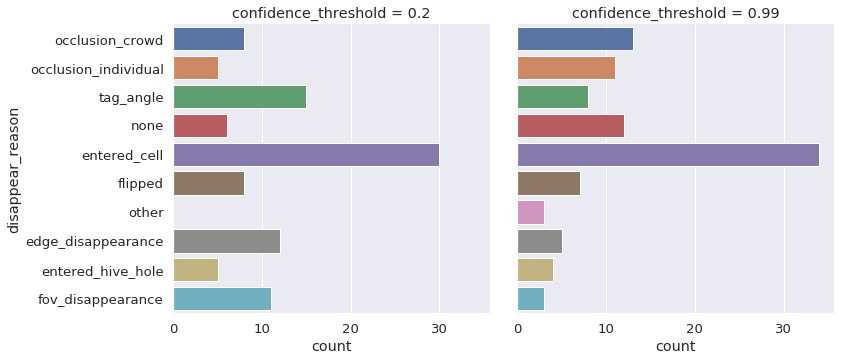
\includegraphics[width=1.0\textwidth]{gap_reason_dist}
\caption[gap_reason_dist]{Reason for disappearance by confidence threshold}
\label{fig:gap_reason_dist}
\end{figure}